\chapter{Specifikacija programske potpore}

\section{Funkcionalni zahtjevi}


\noindent \textbf{Dionici:}

\begin{packed_enum}
	
	\item Studenti
	\item Djelatnici Studentskih centara		
	\item Razvojni tim
	
	
\end{packed_enum}

\noindent \textbf{Aktori i njihovi funkcionalni zahtjevi:}


\begin{packed_enum}
	\item  \underbar{Neregistrirani korisnik (inicijator) može:}
	
	\begin{packed_enum}
		
		\item vidjeti sve oglase
		\item se registrirati, za stvaranje korisničkog računa potrebni su: ime, prezime,korisničko ime, lozinka, e-mail, JMBAG, grad u kojem studira
		
	\end{packed_enum}
	
	\item  \underbar{Registrirani korisnik (inicijator) može:}
	
	\begin{packed_enum}
		
		\item se prijaviti u sustav
		\item stvoriti oglas
		\item vidjeti svoj profil i mijenjati podatke
		\item izbrisati svoj profil
		\item vidjeti oglase pojedinačne ili ulančane koji odgovaraju njegovim kriterijima
		\item pregledati sve svoje oglase (aktivne i neaktivne)
		\item uređivati svoje oglase
		\item učiniti svoje oglase aktivnim i neaktivnim
		\item brisati svoj oglas
		\item "lajkati" oglase po stupnjevima:
		\begin{packed_enum}
			
			\item 1-sviđa mi se
			\item 2-sviđa mi se jako
			\item 3-to je to
			
		\end{packed_enum}
		
	\end{packed_enum}
	
	\item  \underbar{Djelatnik SC-a (inicijator) može:}
	
	\begin{packed_enum}
		\item se prijaviti u sustav
		\item pregledati sve zaključane zamjene
	\end{packed_enum}

	\item  \underbar{Timer (inicijator) može:}
	
	\begin{packed_enum}
		\item pokrenuti uparivanje studenata s oglasima koji odgovaraju njegovim kriterijima
		
	\end{packed_enum}
	
	\item  \underbar{Baza podataka (sudionik):}
	
	\begin{packed_enum}
		\item pohranjuje sve podatke o korisnicima i njihovim ovlastima
		\item pohranjuje sve podatke o oglasima i sobama
	\end{packed_enum}
	
	
	\item  \underbar{Poslužitelj (sudionik):}
	
	\begin{packed_enum}
		\item obrađuje zahtjeve korisnika
		
	\end{packed_enum}
	
	
\end{packed_enum}

\eject 



\subsection{Obrasci uporabe}




\noindent \underbar{\textbf{UC1 -Pregled oglasa}}
\begin{packed_item}
	
	\item \textbf{Glavni sudionik: }Neprijavljeni korisnik
	\item  \textbf{Cilj:}Pregledati oglase soba
	\item  \textbf{Sudionici:} baza podataka
	\item  \textbf{Preduvjet:} 
	\item  \textbf{Opis osnovnog tijeka:}
	
	\item[] \begin{packed_enum}
		
		\item Prilikom otvaranja aplikacije sustav prikazuje sve oglase
		
	\end{packed_enum}
	
	
	
	
\end{packed_item}

\noindent \underbar{\textbf{UC2 -Registracija}}
\begin{packed_item}
	
	\item \textbf{Glavni sudionik: }Neregistrirani korisnik
	\item  \textbf{Cilj:}Registrirati korisnika i ovlastiti ga
	\item  \textbf{Sudionici:} baza podataka, poslužitelj
	\item  \textbf{Preduvjet:} dostupnost poslužitelja, korisnik nije registriran
	\item  \textbf{Opis osnovnog tijeka:}
	
	\item[] \begin{packed_enum}
		
		\item Korisnik pritišće tipku "Registriraj se"
		\item Sustav otvara stranicu za registraciju
		\item Korisnik unosi potrebne podatke
		\item Sustav provjerava ispravnost podataka
		\item Sustav registrira korisnika
		\item Korisnik prima podatke o uspješnoj registraciji
		
	\end{packed_enum}
	
	\item  \textbf{Opis mogućih odstupanja:}
	
	\item[] \begin{packed_item}
		
		\item[2.a]Korisnik unosi neispravne podatke ili već zauzeto korisničko ime ili e-mail
		\item[] \begin{packed_enum}
			
			\item Sustav obavještava korisnika o pogrešci 
			\item Sustav vraća korisnika na stranicu za registraciju sa crveno označenom greškom
			\item Korisnik mijenja neispravne podatke te završava unos ili odustaje od registracije
			
		\end{packed_enum}
		
	\end{packed_item}
\end{packed_item}

\noindent \underbar{\textbf{UC3 -Prijava u sustav}}
\begin{packed_item}
	
	\item \textbf{Glavni sudionik: }Registrirani korisnik, Djelatnik SC-a
	\item  \textbf{Cilj:}Prijaviti se u sustav
	\item  \textbf{Sudionici:} baza podataka
	\item  \textbf{Preduvjet:} Korisnik se je registrirao
	\item  \textbf{Opis osnovnog tijeka:}
	
	\item[] \begin{packed_enum}
		
		\item Unos korisničkog imena i lozinke
		\item Sustav provjerava ispravnost podataka
		\item Sustav korisniku otvara početnu stranicu i korisnik ima pristup korisničkim funkcijama
	\end{packed_enum}
	
	\item  \textbf{Opis mogućih odstupanja:}
	
	\item[] \begin{packed_item}
		
		\item[2.a] Unos neispravnih podataka
		\item[] \begin{packed_enum}
			
			\item  Sustav obavještava o neispravnim podacima i vraća na stanicu za prijavu s crveno označenom pogreškom
			\item Korisnik ispravlja podatke
			
			
		\end{packed_enum}
		
	\end{packed_item}
\end{packed_item}

\noindent \underbar{\textbf{UC4 -Objavljivanje oglasa}}
\begin{packed_item}
	
	\item \textbf{Glavni sudionik: }Prijavljeni korisnik
	\item  \textbf{Cilj:}Objaviti oglas
	\item  \textbf{Sudionici:} baza podataka,poslužitelj
	\item  \textbf{Preduvjet:} Korisnik je prijavljen u sustav
	\item  \textbf{Opis osnovnog tijeka:}
	
	\item[] \begin{packed_enum}
		
		\item Korisnik odabire opciju "Objavi novi oglas"
		\item Sustav otvara stranicu za objavljivanje oglasa
		\item Korisnik upisuje potrebne podatke za sobu koju nudi i kriterije za sobu koju traži. Sve podatke odabire iz padajućih izbornika osim polja za proizvoljni komentar
		\item Korisnik pritišće tipku "objavi" 
		\item Sustav pohranjuje oglas u bazu
	\end{packed_enum}
	
\end{packed_item}

\noindent \underbar{\textbf{UC5 -Pregled mogućih zamjena }}
\begin{packed_item}
	
	\item \textbf{Glavni sudionik: }Prijavljeni korisnik
	\item  \textbf{Cilj:}Pregledati ponuđene moguće zamjene koje odgovaraju kriterijima korisnika
	\item  \textbf{Sudionici:} baza podataka, poslužitelj
	\item  \textbf{Preduvjet:} Korisnik je prijavljen i ima aktivan oglas
	\item  \textbf{Opis osnovnog tijeka:}
	
	\item[] \begin{packed_enum}
		
		\item Korisnik otvara početnu stranicu
		\item Sustav prikazuje sve oglase koji odgovaraju njegovim kriterijima
		
	\end{packed_enum}
\end{packed_item}
\noindent \underbar{\textbf{UC6 - Uparivanje oglasa}}
\begin{packed_item}
	
	\item \textbf{Glavni sudionik: }Timer
	\item  \textbf{Cilj:}Upariti studenta s oglasima koji odgovaraju njegovim kriterijima
	\item  \textbf{Sudionici:} baza podataka, poslužitelj
	\item  \textbf{Preduvjet:}
	\item  \textbf{Opis osnovnog tijeka:}
	
	\item[] \begin{packed_enum}
		
		\item Timer pokreće uparivanje svakih 5 sati
		\item Sustav za svakog studenta stvara listu svih oglasa koji direktno ili lančano odgovaraju njegovim kriterijima
		
	\end{packed_enum}
\end{packed_item}

\noindent \underbar{\textbf{UC7 -Lajkanje oglasa}}
\begin{packed_item}
	
	\item \textbf{Glavni sudionik: }Prijavljeni korisnik
	\item  \textbf{Cilj:}"Lajkati" oglase soba koje korisnika zanimaju
	\item  \textbf{Sudionici:} baza podataka, poslužitelj
	\item  \textbf{Preduvjet:} Korisnik je prijavljen, ima aktivan oglas i barem jedan oglas odgovara njegovim kriterijima
	\item  \textbf{Opis osnovnog tijeka:}
	
	\item[] \begin{packed_enum}
		
		\item Korisnik oglase koji ga zanimaju označava("lajka") po stupnjevima od 1 do 3
		\item Sustav sprema njegov odabir
	\end{packed_enum}
	
\end{packed_item}

\noindent \underbar{\textbf{UC8 -Mjenjanje Lajka}}
\begin{packed_item}
	
	\item \textbf{Glavni sudionik: }Prijavljeni korisnik
	\item  \textbf{Cilj:}Promijeniti razinu "lajka" ili maknuti lajk
	\item  \textbf{Sudionici:} baza podataka, poslužitelj
	\item  \textbf{Preduvjet:} Korisnik je prijavljen, ima aktivan oglas,barem jedan oglas odgovara njegovim kriterijima
	\item  \textbf{Opis osnovnog tijeka:}
	
	\item[] \begin{packed_enum}
		
		\item Korisnik odabire neki drugi stupanj "lajka" ili odustaje od "lajka" micanjem oznake
		\item Njegov odabir se sprema u bazu podataka
		
	\end{packed_enum}
	
\end{packed_item}

\noindent \underbar{\textbf{UC9 -Pregled mojih oglasa}}
\begin{packed_item}
	
	\item \textbf{Glavni sudionik: }Prijavljeni korisnik
	\item  \textbf{Cilj:}Vidjeti sve svoje oglase
	\item  \textbf{Sudionici:} baza podataka, poslužitelj
	\item  \textbf{Preduvjet:} Korisnik je prijavljen i ima oglas
	\item  \textbf{Opis osnovnog tijeka:}
	
	\item[] \begin{packed_enum}
		
		\item Korisnik odabire opciju "Moji oglasi"
		\item Sustav otvara stranicu gdje se prikazuju svi korisnikovi oglasi
		
	\end{packed_enum}
\end{packed_item}

\noindent \underbar{\textbf{UC10 -Uređivanje oglasa}}
\begin{packed_item}
	
	\item \textbf{Glavni sudionik: }Prijavljeni korisnik
	\item  \textbf{Cilj:}Urediti već postojeći oglas
	\item  \textbf{Sudionici:} baza podataka, poslužitelj
	\item  \textbf{Preduvjet:} Korisnik je prijavljen i ima aktivan oglas
	\item  \textbf{Opis osnovnog tijeka:}
	
	\item[] \begin{packed_enum}
		
		\item Korisnik odlazi pod "Moji oglasi" 
		\item Sustav prikazuje stranicu sa listom njegovih oglasa
		\item Korisnik odabire opciju uredi
		\item Korisnik mijenja podatke ili atribut je li oglas aktivan ili neaktivan
		\item Korisnik potvrđuje promjene odabirom opcije spremi
		\item Promjene se spremaju u bazu podataka 
		
	\end{packed_enum}
\end{packed_item}



\noindent \underbar{\textbf{UC11 -Brisanje oglasa}}
\begin{packed_item}
	
	\item \textbf{Glavni sudionik: }Prijavljeni korisnik
	\item  \textbf{Cilj:}Izbrisati oglas
	\item  \textbf{Sudionici:} baza podataka, poslužitelj
	\item  \textbf{Preduvjet:} Korisnik je prijavljen i ima oglas
	\item  \textbf{Opis osnovnog tijeka:}
	
	\item[] \begin{packed_enum}
		
		\item Korisnik odlazi pod "Moji oglasi" 
		\item Sustav prikazuje stranicu sa listom njegovih oglasa
		\item Korisnik odabire opciju izbriši
		\item Sustav briše oglas iz baze podataka
		
	\end{packed_enum}
\end{packed_item}

\noindent \underbar{\textbf{UC12 -Pregled profila}}
\begin{packed_item}
	
	\item \textbf{Glavni sudionik: }Prijavljeni korisnik
	\item  \textbf{Cilj:}Vidjeti svoje osobne podatke
	\item  \textbf{Sudionici:} baza podataka, poslužitelj
	\item  \textbf{Preduvjet:} Korisnik je prijavljen
	\item  \textbf{Opis osnovnog tijeka:}
	
	\item[] \begin{packed_enum}
		
		\item Korisnik odlazi pod "Moj profil"
		\item Sustav otvara stranicu korisnikova profila 
		
	\end{packed_enum}
\end{packed_item}

\noindent \underbar{\textbf{UC13 -Promjena profila}}
\begin{packed_item}
	
	\item \textbf{Glavni sudionik: }Prijavljeni korisnik
	\item  \textbf{Cilj:}Vidjeti svoje osobne podatke
	\item  \textbf{Sudionici:} baza podataka, poslužitelj
	\item  \textbf{Preduvjet:} Korisnik je prijavljen
	\item  \textbf{Opis osnovnog tijeka:}
	
	\item[] \begin{packed_enum}
		
		\item Korisnik odlazi pod "Moj profil"
		\item Sustav otvara stranicu korisnikova profila 
		\item Korisnik odabire opciju "uredi"
		\item Korisnik mijenja osobne podatke
		\item Korisnik pritišće tiku "spremi promjene"
		\item Sustav sprema promjene 
		
	\end{packed_enum}
\end{packed_item}

\noindent \underbar{\textbf{UC14 -Brisanje profila}}
\begin{packed_item}
	
	\item \textbf{Glavni sudionik: }Prijavljeni korisnik
	\item  \textbf{Cilj:}Vidjeti svoje osobne podatke
	\item  \textbf{Sudionici:} baza podataka, poslužitelj
	\item  \textbf{Preduvjet:} Korisnik je prijavljen
	\item  \textbf{Opis osnovnog tijeka:}
	
	\item[] \begin{packed_enum}
		
		\item Korisnik odlazi pod "Moj profil"
		\item Sustav otvara stranicu korisnikova profila 
		\item Korisnik odabire opciju "izbriši profil"
		\item Sustav briše korisnikov profil i otvara početnu stranicu
		
	\end{packed_enum}
\end{packed_item}

\noindent \underbar{\textbf{UC15 -Potvrđivanje zamjene}}
\begin{packed_item}
	
	\item \textbf{Glavni sudionik: }Prijavljeni korisnik
	\item  \textbf{Cilj:}Potvrditi zamjenu sobe
	\item  \textbf{Sudionici:} baza podataka, poslužitelj
	\item  \textbf{Preduvjet:} Korisnik je prijavljen, sve uključene strane su "lajkale" oglas
	\item  \textbf{Opis osnovnog tijeka:}
	
	\item[] \begin{packed_enum}
		
		\item Korisnik dobiva obavijest da su sve strane "lajkale" zamjenu
		\item Korisnik pomoću linka iz obavijesti dolazi do oglasa
		\item Korisnik potvrđuje zamjenu
		\item Potvrda se sprema u bazu podataka
		
	\end{packed_enum}
\end{packed_item}
\noindent \underbar{\textbf{UC16 -Pregled zaključanih zamjena}}
\begin{packed_item}
	
	\item \textbf{Glavni sudionik: }Djelatnik SC-a
	\item  \textbf{Cilj:}Vidjeti sve zaključane zamjene kako bi se mogle provesti u sustavu SC-a
	\item  \textbf{Sudionici:} baza podataka, poslužitelj
	\item  \textbf{Preduvjet:}Djelatnik je prijavljen
	\item  \textbf{Opis osnovnog tijeka:}
	
	\item[] \begin{packed_enum}
		
		\item Sustav na početnoj stranici prikazuje listu svih zaključanih zamjena
		\item Korisnik označuje sve zamjene koje je proveo
		\item Sustav miče označene zamjene sa stranice
		
		
	\end{packed_enum}
	
\end{packed_item}	
\noindent \underbar{\textbf{UC17 -Odjava}}
\begin{packed_item}
	
	\item \textbf{Glavni sudionik: }Djelatnik SC-a, Prijavljeni korisnik
	\item  \textbf{Cilj:}Odjaviti se iz sustava
	\item  \textbf{Sudionici:}poslužitelj
	\item  \textbf{Preduvjet:}Djelatnik je prijavljen
	\item  \textbf{Opis osnovnog tijeka:}
	
	\item[] \begin{packed_enum}
		
		\item Korisnik pritišće tipku "odjavi se"
		\item Sustav odjavljuje korisnika te otvara početnu stranicu		
		
	\end{packed_enum}
	
\end{packed_item}	

\noindent \textbf{Dijagrami obrazaca uporabe}
\begin{figure}[H]
	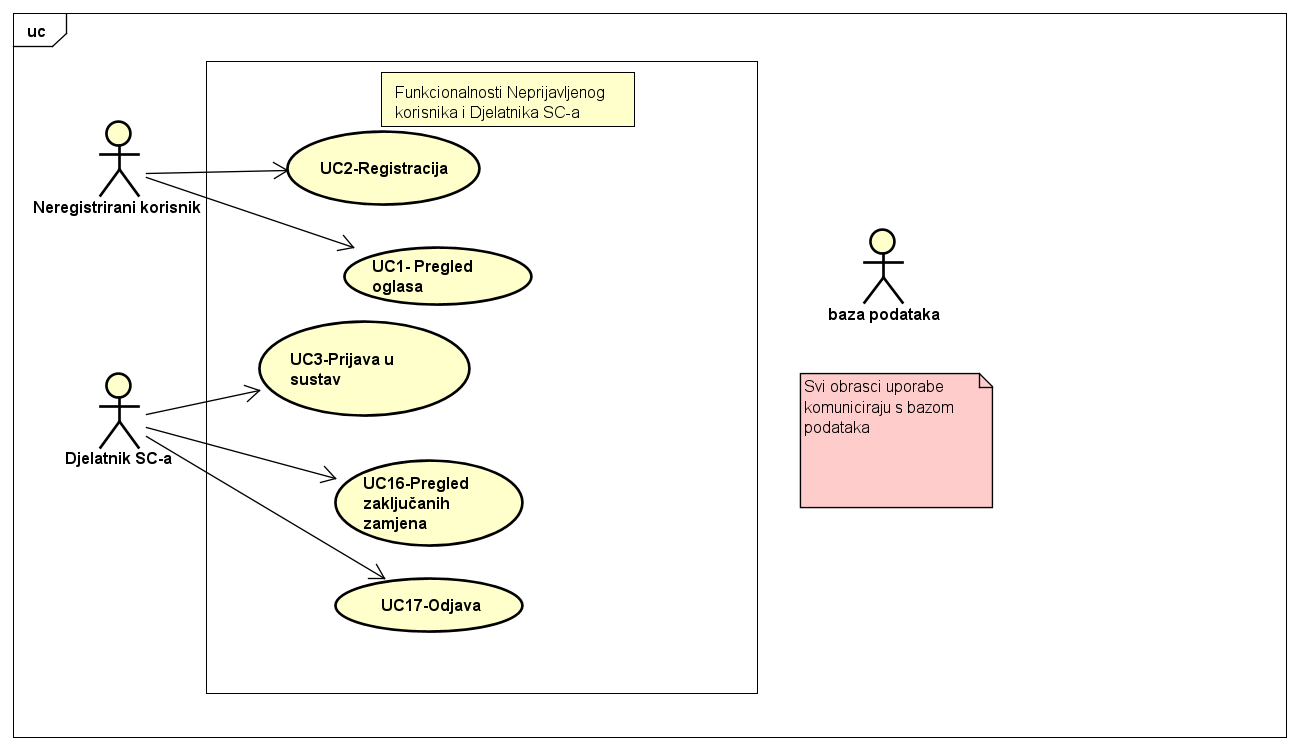
\includegraphics[scale=0.4]{dijagrami/dijagram1.PNG} %veličina slike u odnosu na originalnu datoteku i pozicija slike
	\centering
	\caption{Dijagrami obrazaca uporabe, funkcionalnost neregistriranog korisnika i djelatnika SC-a}
	\label{fig:dijagramObrazaca1}
\end{figure}

\begin{figure}[H]
	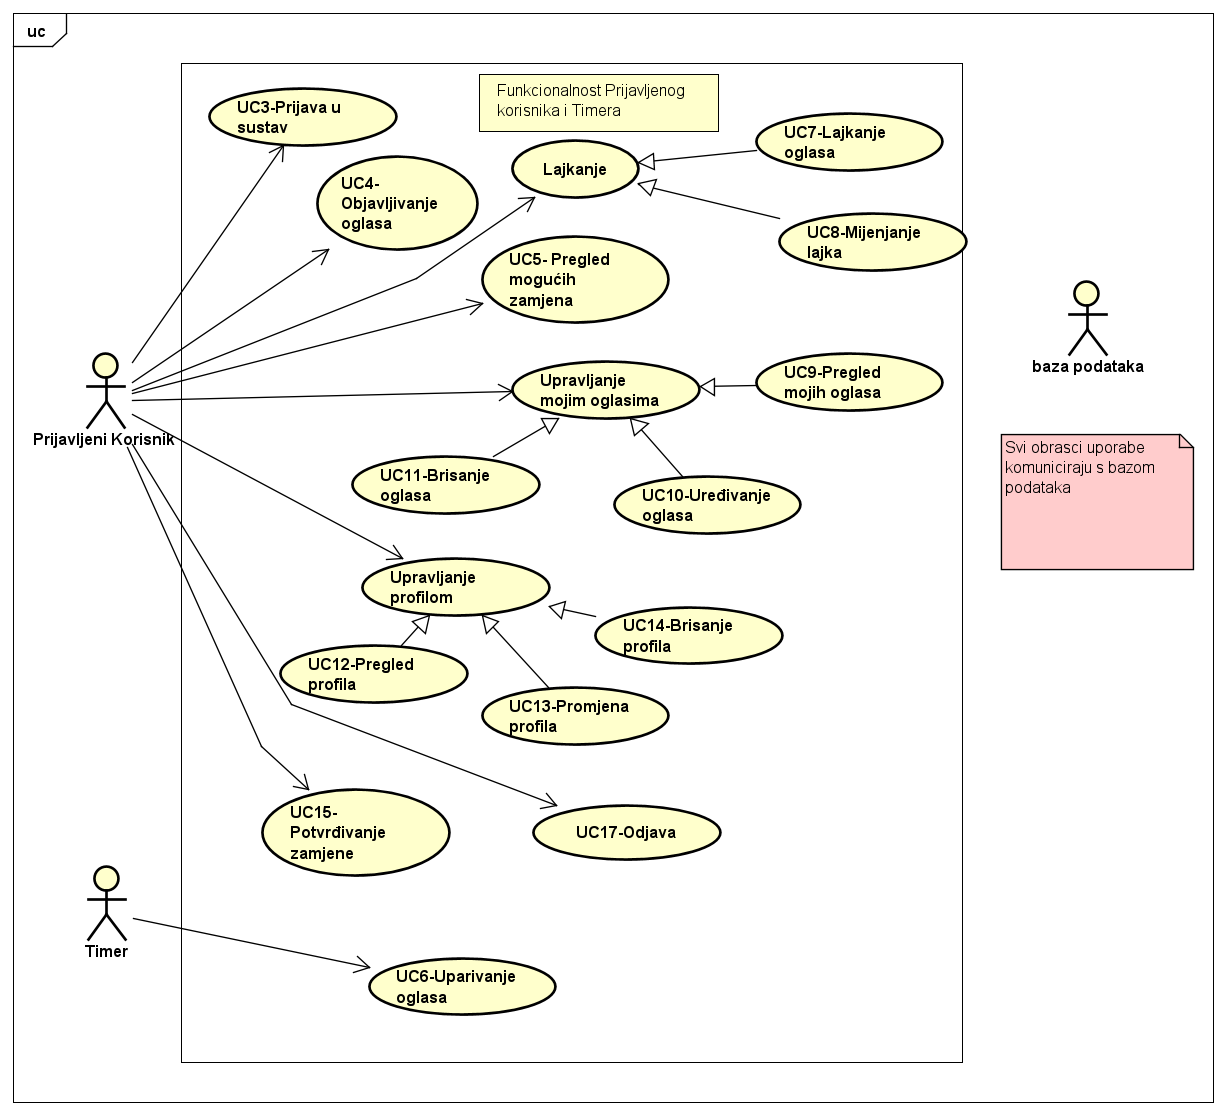
\includegraphics[scale=0.4]{dijagrami/dijagram2.PNG} %veličina slike u odnosu na originalnu datoteku i pozicija slike
	\centering
	\caption{Dijagrami obrazaca uporabe, funkcionalnost prijavljenog korisnika i timera}
	\label{fig:dijagramObrazaca2}
\end{figure}

\eject

\subsection{Sekvencijski dijagrami}

\noindent \textbf{Obrazac uporabe UC3(Prijava u sustav)}\\
	\indent Neprijavljeni korisnik šalje zahtjev za prijavu s korisničkim imenom i lozinkom. Provjerava se ako je korisničko ime u bazi podataka. Ako ime ne postoji dojavljuje se greška u suprotnom provjerava se ako mu odgovara unesena lozinka. Ako lozinka odgovara tada se korisniku dodjeljuju ovlasti u suprotnom se dojavljuje greška.


\begin{figure}[H]
	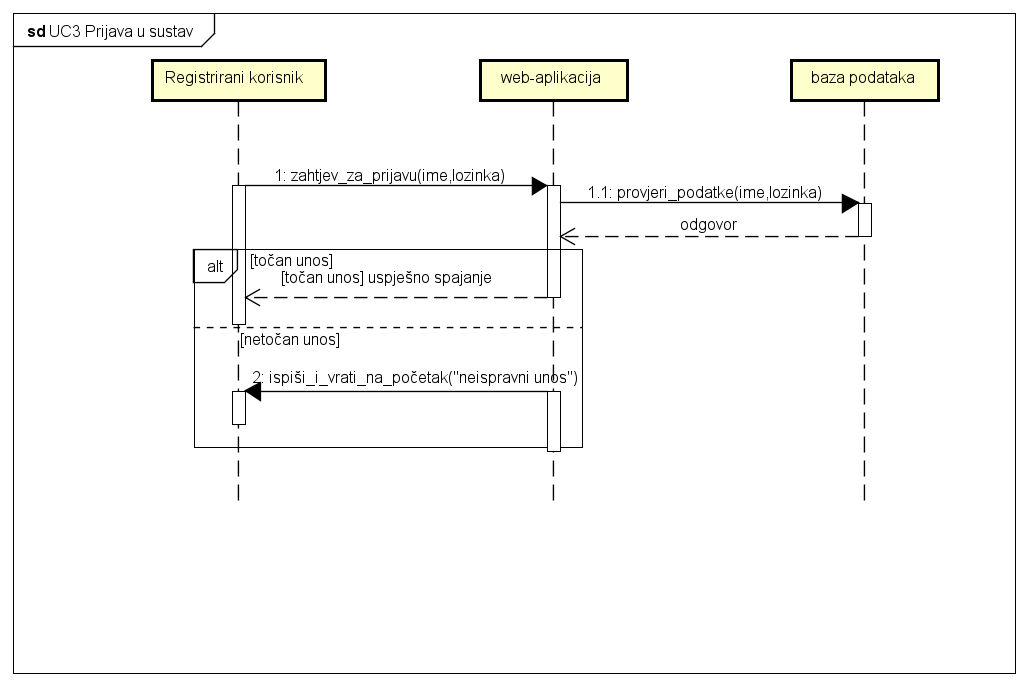
\includegraphics[scale=0.4]{dijagrami/UC3 Prijava u sustav.PNG} %veličina slike u odnosu na originalnu datoteku i pozicija slike
	\centering
	\caption{Sekvencijski dijagram za UC3}
	\label{fig:sekdijag1}
\end{figure}

\noindent \textbf{Obrazac uporabe UC4(Objavljivanje oglasa)}\\
\indent Korisnik odabire opciju "Objavi novi oglas". Zatim u obrascu iz padajućih izbornika bira grad zatim mu se nude svi domovi. Nakon odabira doma prikazuju mu se paviljoni i tako dalje za kat i broj sobe. Zatim korisnik označava iste  kriterije za sobu koju traži. Pritiskom na oznaku spremi sprema se oglas u bazu podataka.



\begin{figure}[H]
	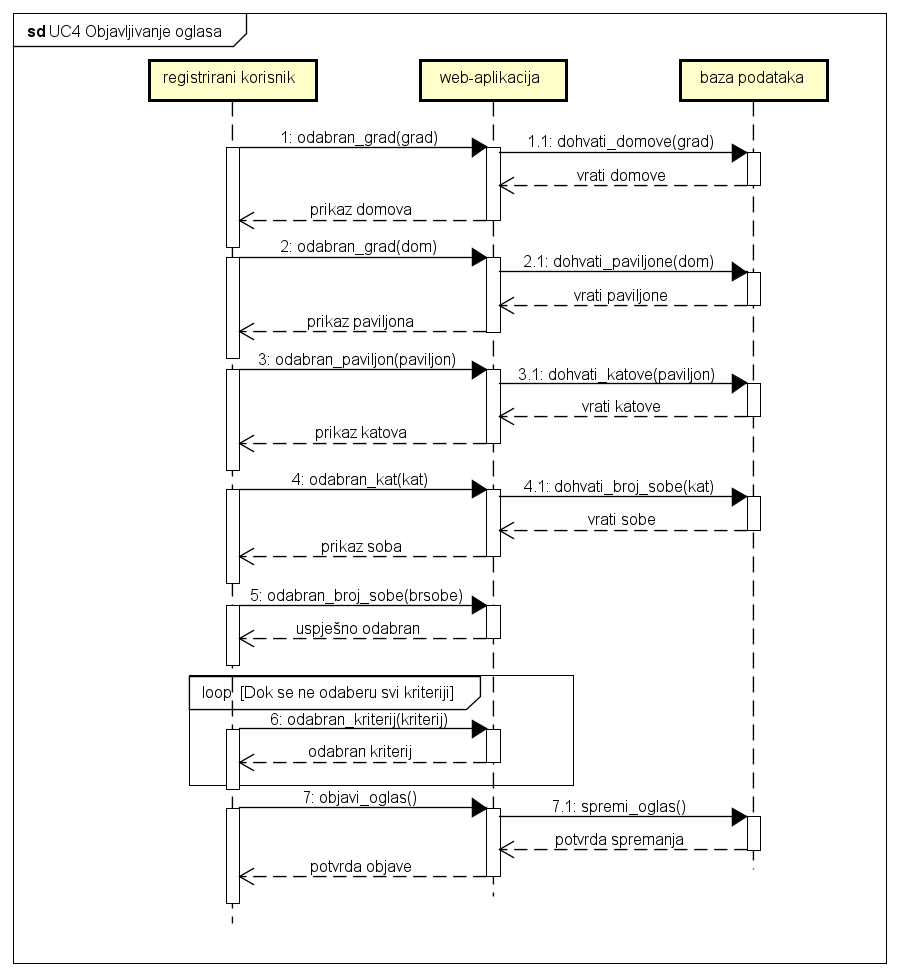
\includegraphics[scale=0.4]{dijagrami/UC4 Objavljivanje oglasa.PNG} %veličina slike u odnosu na originalnu datoteku i pozicija slike
	\centering
	\caption{Sekvencijski dijagram za UC4}
	\label{fig:sekdijag2}
\end{figure}

\noindent \textbf{Obrazac uporabe UC5(Pregled mogućih zamjena)}\\
\indent Korisnik nakon što napravi oglas odlazi na početnu stranicu gdje dobiva listu svih oglasa koji odgovaraju njegovim kriterijima.


\begin{figure}[H]
	\includegraphics[scale=0.4]{dijagrami/UC5 Pregled mogućih zamjena.PNG} %veličina slike u odnosu na originalnu datoteku i pozicija slike
	\centering
	\caption{Sekvencijski dijagram za UC5}
	\label{fig:sekdijag3}
\end{figure}

\noindent \textbf{Obrazac uporabe UC15(Potvrđivanje zamjene)}\\
\indent Korisnik potvrđuje zamjenu odabirom opcije "zaključaj zamjenu". Potvrda se sprema u bazu podataka promjenom statusa oglasa tek kad sve strane potvrde zamjenu.


\begin{figure}[H]
	\includegraphics[scale=0.4]{dijagrami/UC15 Potvrđivanje zamjene.PNG} %veličina slike u odnosu na originalnu datoteku i pozicija slike
	\centering
	\caption{Sekvencijski dijagram za UC15}
	\label{fig:sekdijag4}
\end{figure}

\section{Ostali Zahtjevi}
\begin{packed_enum}
	\item Sustav treba omogućiti rad više korisnika u stvarnom vremenu
	\item Sustav bi se trebao moći koristiti bez dodatnih uputa
	\item Sustav i korisničko sučelje trebaju podržavati hrvatsku abecedu
	\item Izvršavanje dijela programa u kojem se pristupa bazi podataka ne smije trajati duže od nekoliko sekundi
	\item Neispravno korištenje korisničkog sučelja ne smije narušiti funkcionalnost i rad sustava
	\item Nadogradnja sustava ne smije narušavati postojeće funkcionalnosti sustava
	\item Aplikacija treba biti izvedena kao web aplikacija prilagođena (engl. responsive) mobilnom uređaju
\end{packed_enum}



